\begin{mychapter}{Interfaccia Utente (UI/UX)}

\begin{mysection}{Design e Suddivisione dei Ruoli}
L'interfaccia utente di Scalamarket separa l'esperienza dell'utente finale (il Cliente) da quella degli operatori di back-office (gli Amministratori/Gestori Filiera), mantenendo un'architettura frontend unificata. Il design adotta uno stile moderno, caratterizzato da temi scuri (Dark Mode), palette di colori vivaci e layout responsivo.

\begin{figure}[H]
    \centering
    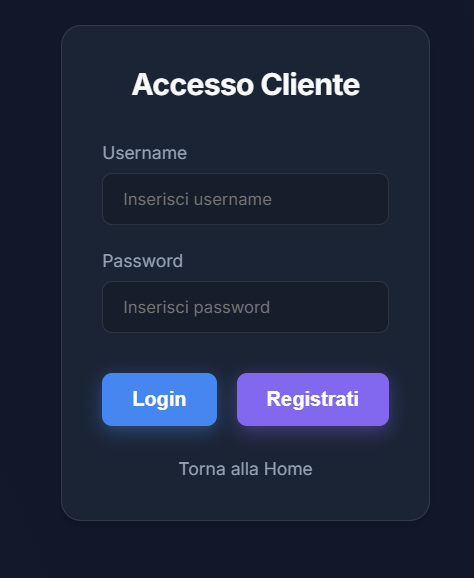
\includegraphics[width=\textwidth,height=0.45\textheight,keepaspectratio]{img/client_login.png}
    \caption{Schermata di Accesso e Registrazione (Area Clienti)}
    \label{fig:client_login}
\end{figure}

L'area di back-office, invece, offre un sistema di registrazione basato su ruoli: è possibile iscriversi come Amministratore Globale, per una supervisione totale della piattaforma, oppure come Gestore Filiale, con la facoltà di selezionare una delle tre filiali operative disponibili al momento dell'iscrizione.

\begin{figure}[H]
    \centering
    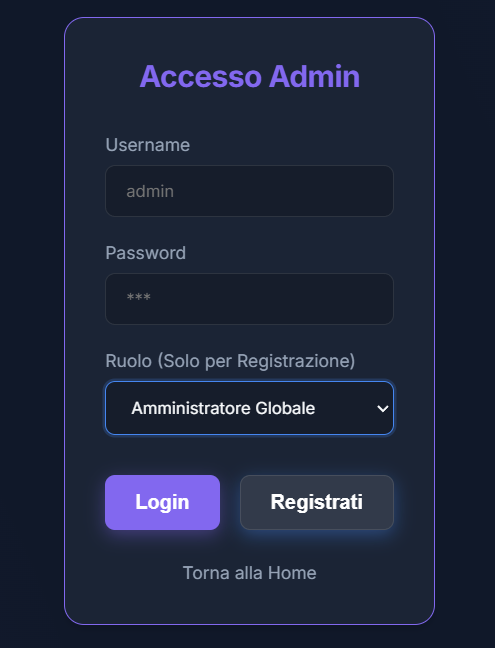
\includegraphics[width=\textwidth,height=0.45\textheight,keepaspectratio]{img/register_global_admin.png}
    \caption{Registrazione di un nuovo Amministratore Globale}
    \label{fig:register_global_admin}
\end{figure}

\begin{figure}[H]
    \centering
    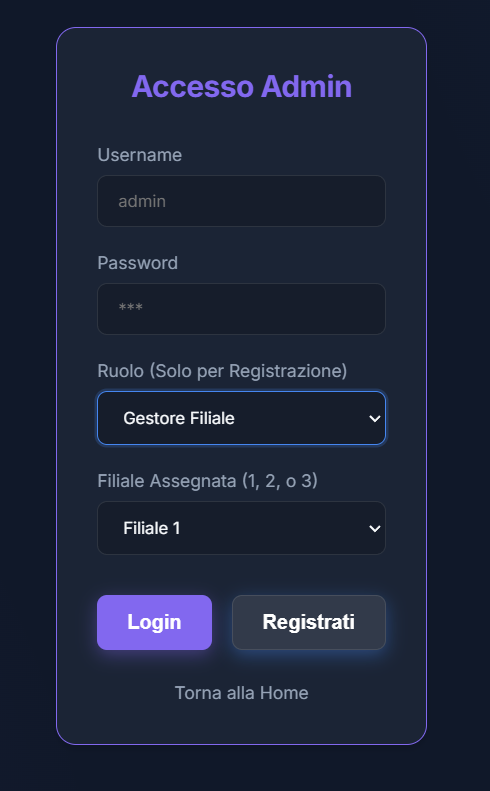
\includegraphics[width=\textwidth,height=0.45\textheight,keepaspectratio]{img/register_local_admin.png}
    \caption{Registrazione di un Gestore Filiale con scelta della sede}
    \label{fig:register_local_admin}
\end{figure}

Si precisa che gli attuali moduli di autenticazione e registrazione, sebbene pienamente funzionali ai fini dell'illustrazione delle dinamiche di accesso basate sui ruoli (RBAC), sono stati concepiti come \textit{Proof of Concept} (PoC) per dimostrare le capacità architetturali e di routing della piattaforma. Tali schermate e le relative implementazioni lato client risultano pertanto semplificate; per un effettivo rilascio in ambiente di produzione (\textit{enterprise}), si renderebbe necessaria l'integrazione di strati di sicurezza più avanzati, policy di password complesse, validazione multi-fattore (MFA) e sistemi di Identity Access Management (IAM) dedicati.
\end{mysection}

\begin{mysection}{Pannello Cliente}
La dashboard cliente mostra il catalogo degli articoli, con disponibilità residua globale calcolata dinamicamente interrogando il servizio inventario. Il carrello impedisce l'aggiunta di quantità superiori alla disponibilità.

\begin{figure}[H]
    \centering
    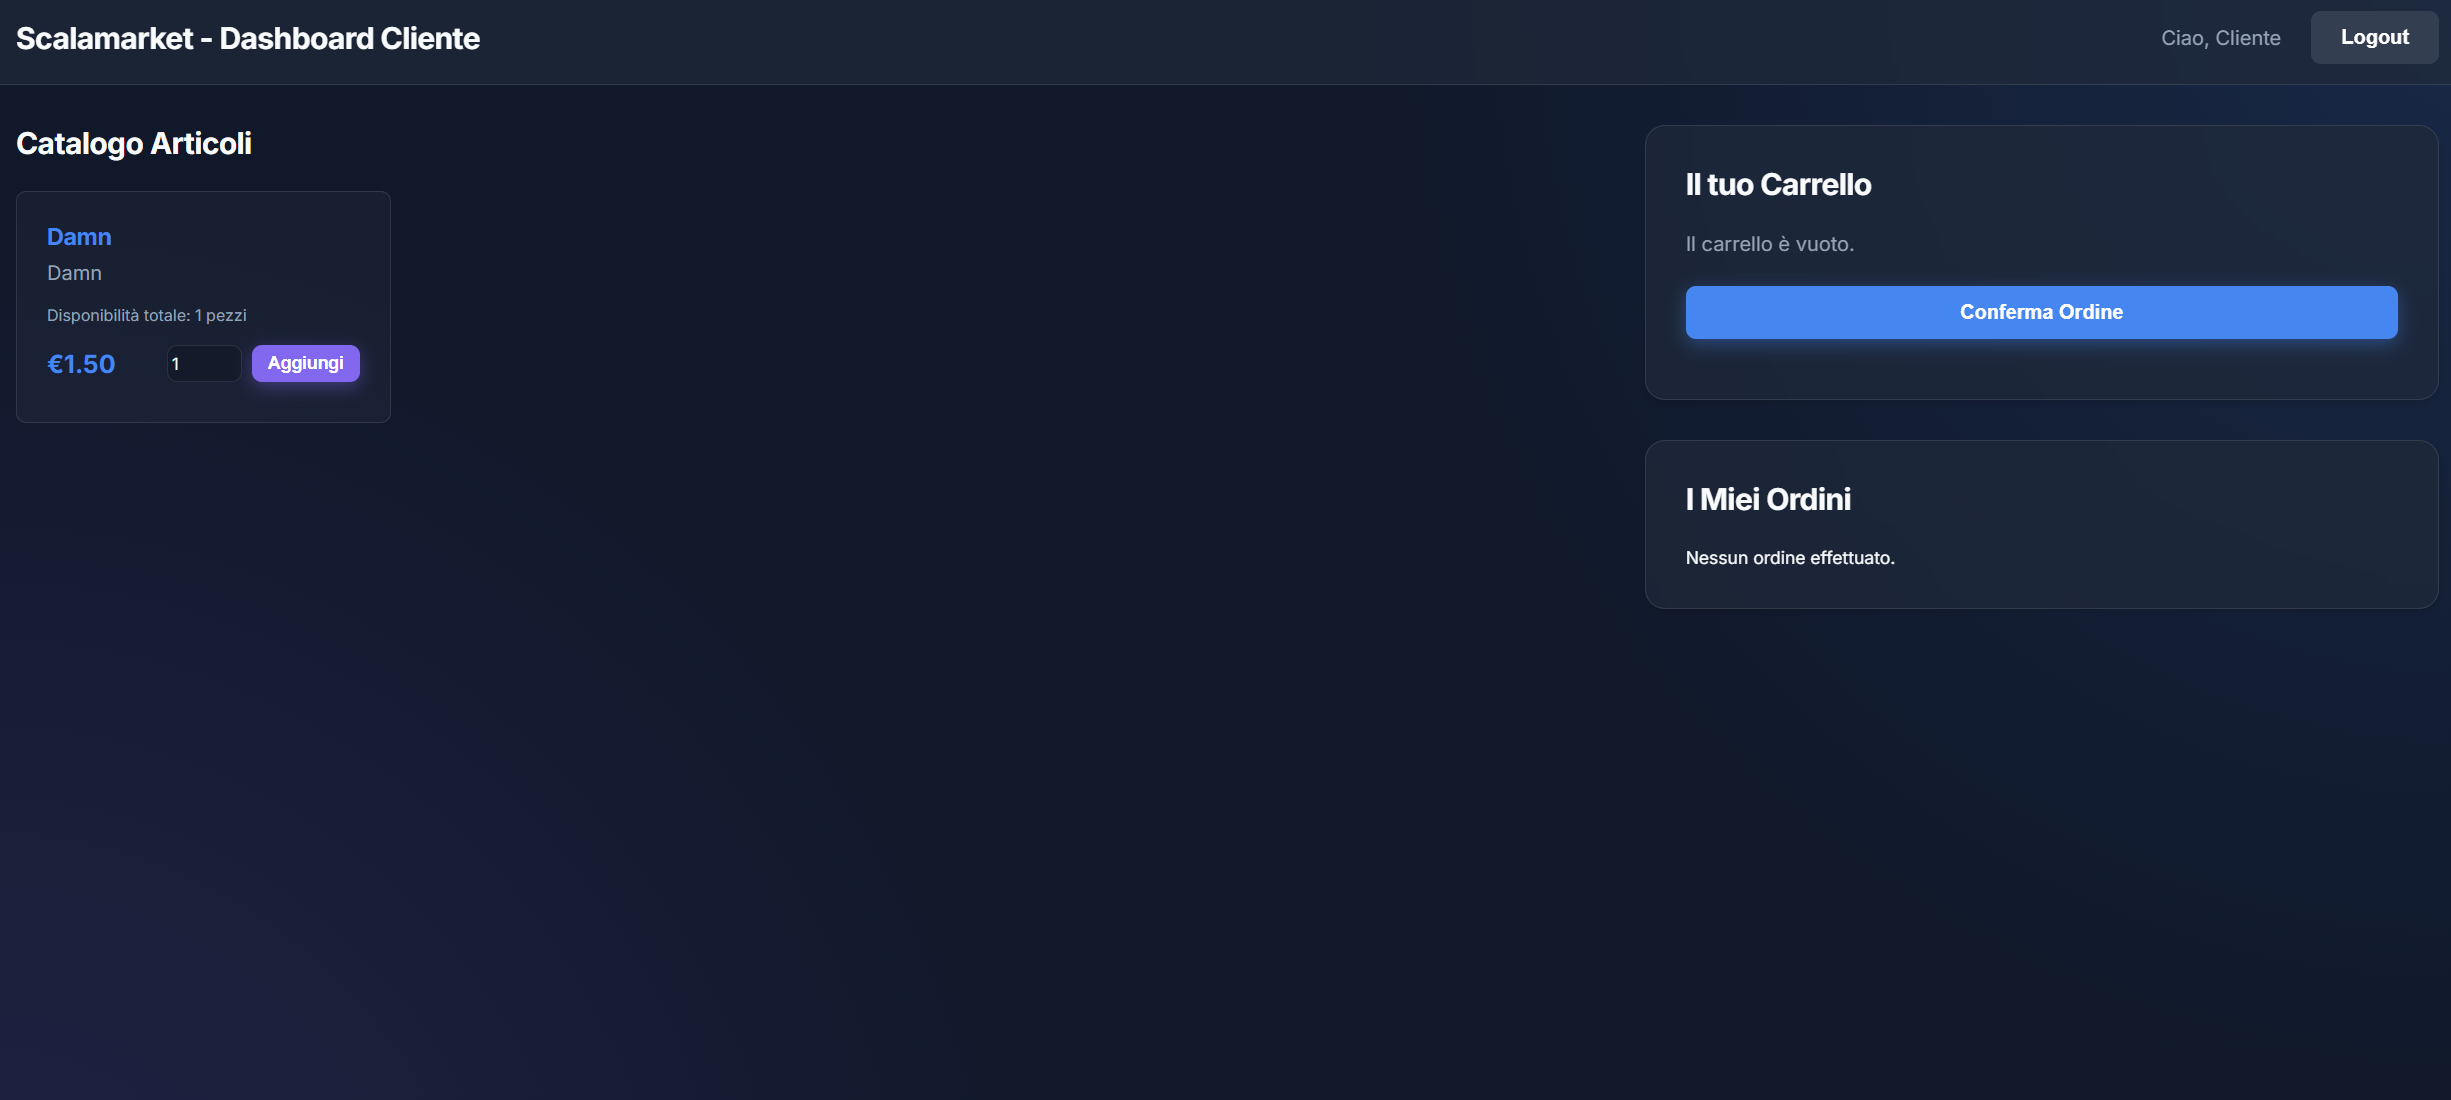
\includegraphics[width=\textwidth,height=0.45\textheight,keepaspectratio]{img/client_catalog.png}
    \caption{Dashboard Cliente: Catalogo Prodotti e Carrello}
    \label{fig:client_catalog}
\end{figure}

\begin{figure}[H]
    \centering
    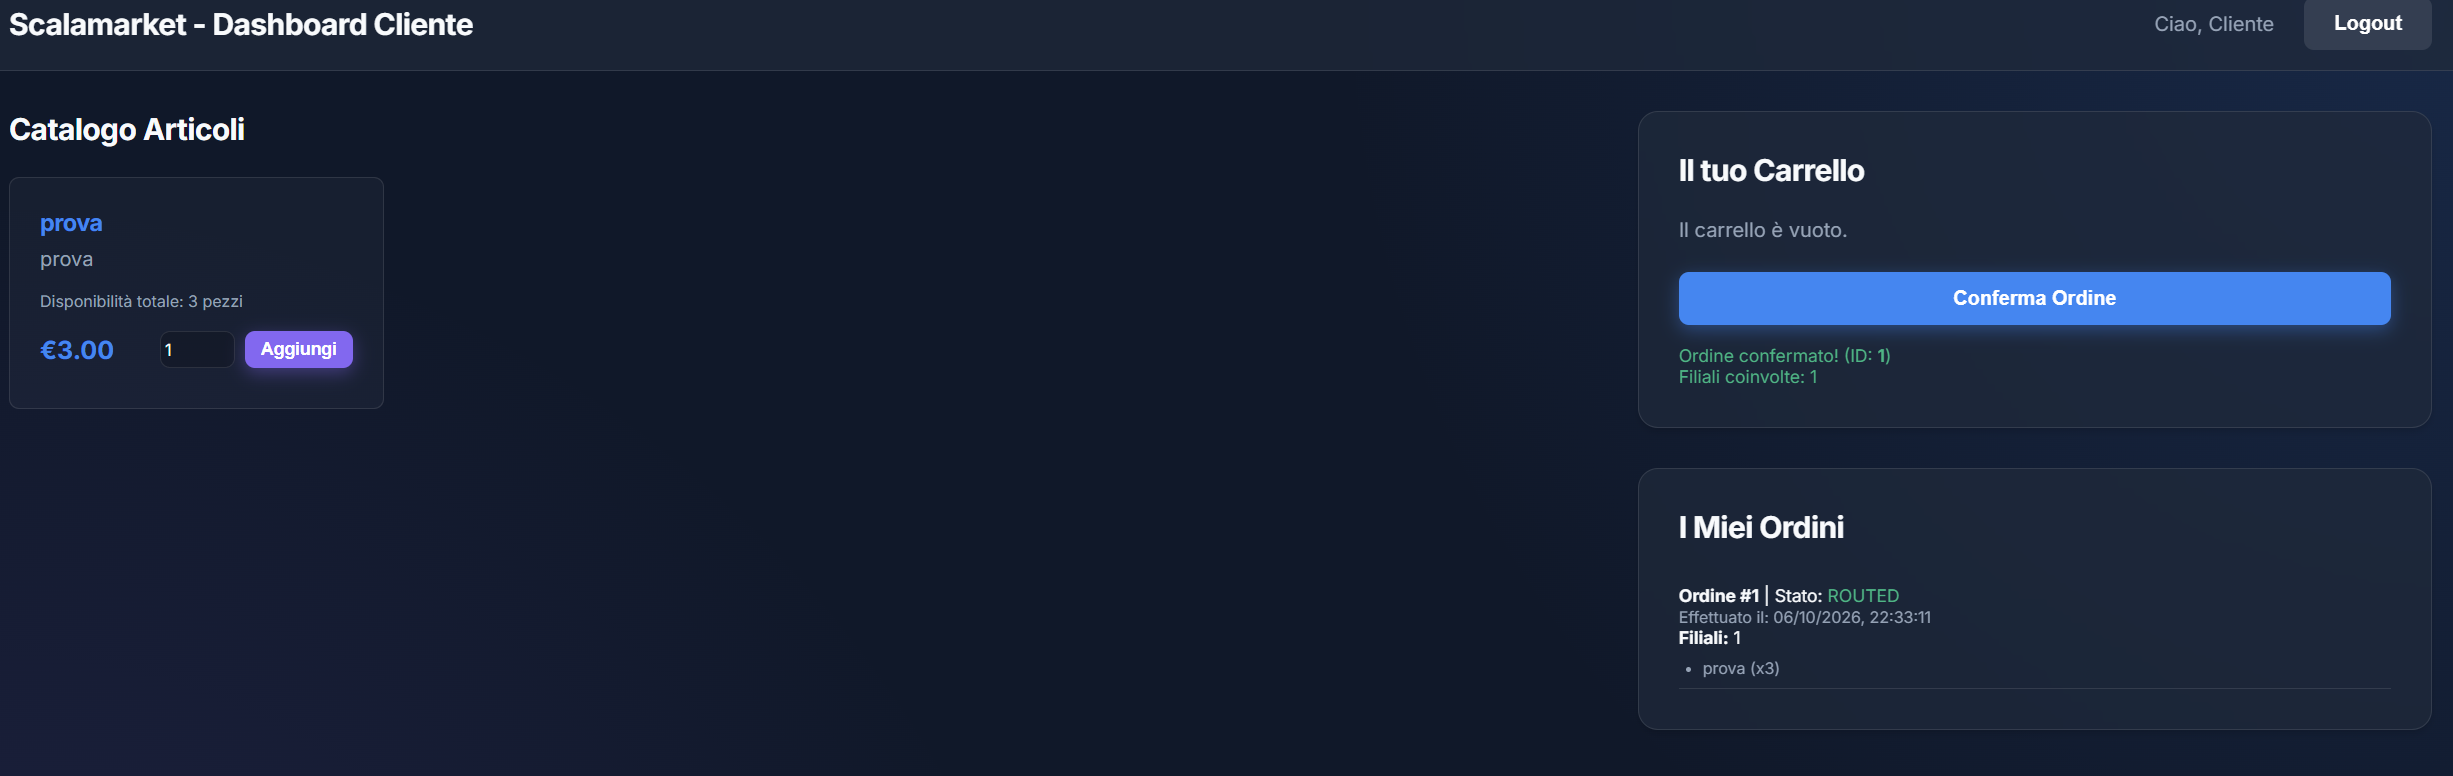
\includegraphics[width=\textwidth,height=0.45\textheight,keepaspectratio]{img/successful_order_client.png}
    \caption{Conferma dell'ordine andato a buon fine (Area Cliente)}
    \label{fig:successful_order_client}
\end{figure}
\end{mysection}

\begin{mysection}{Pannelli di Amministrazione}
Accedendo alla dashboard di amministrazione, gli operatori e i gestori di filiera hanno a disposizione sezioni specifiche per l'aggiunta di nuovi articoli, la gestione logistica (aggiornamento dei mezzi di trasporto) e l'inventario globale consolidato.

\begin{figure}[H]
    \centering
    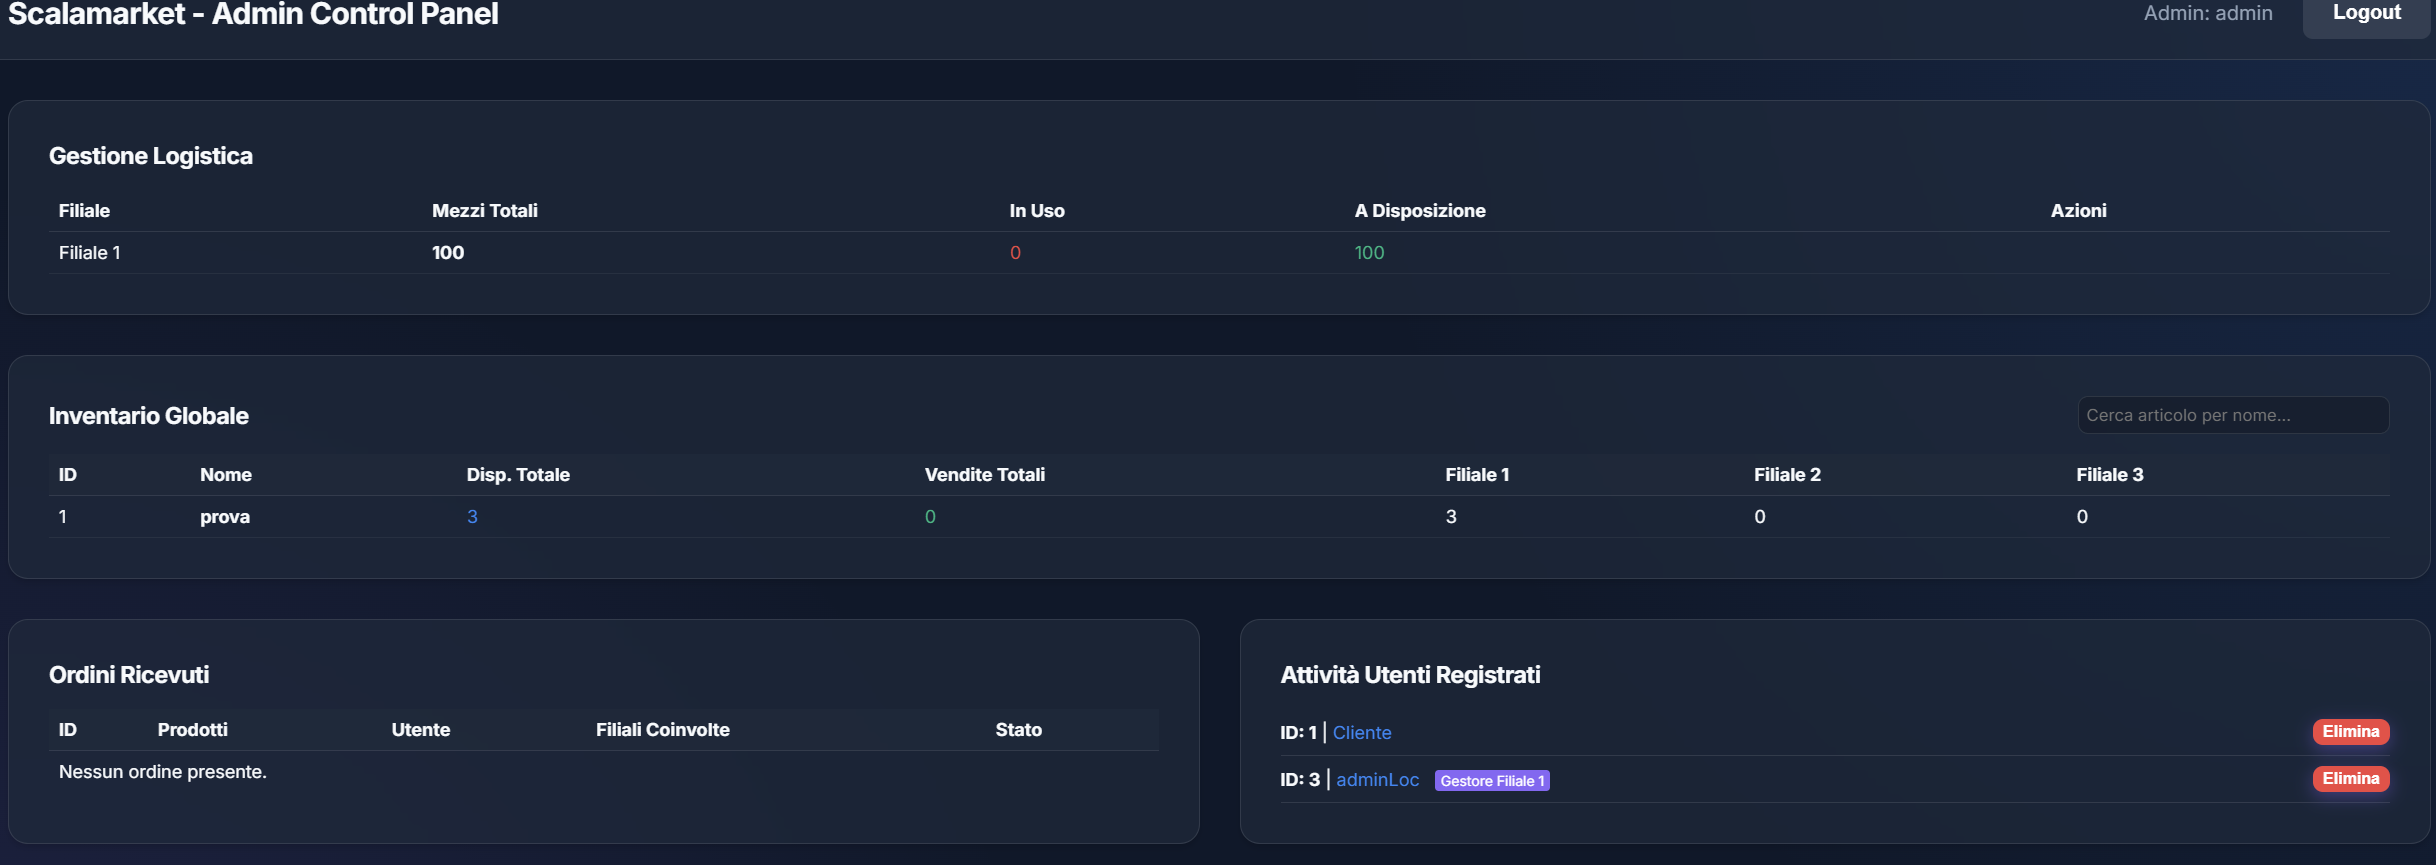
\includegraphics[width=\textwidth,height=0.45\textheight,keepaspectratio]{img/admin_dashboard.png}
    \caption{Dashboard Amministratore (Inventario, Logistica e Analytics)}
    \label{fig:admin_dashboard}
\end{figure}

\begin{figure}[H]
    \centering
    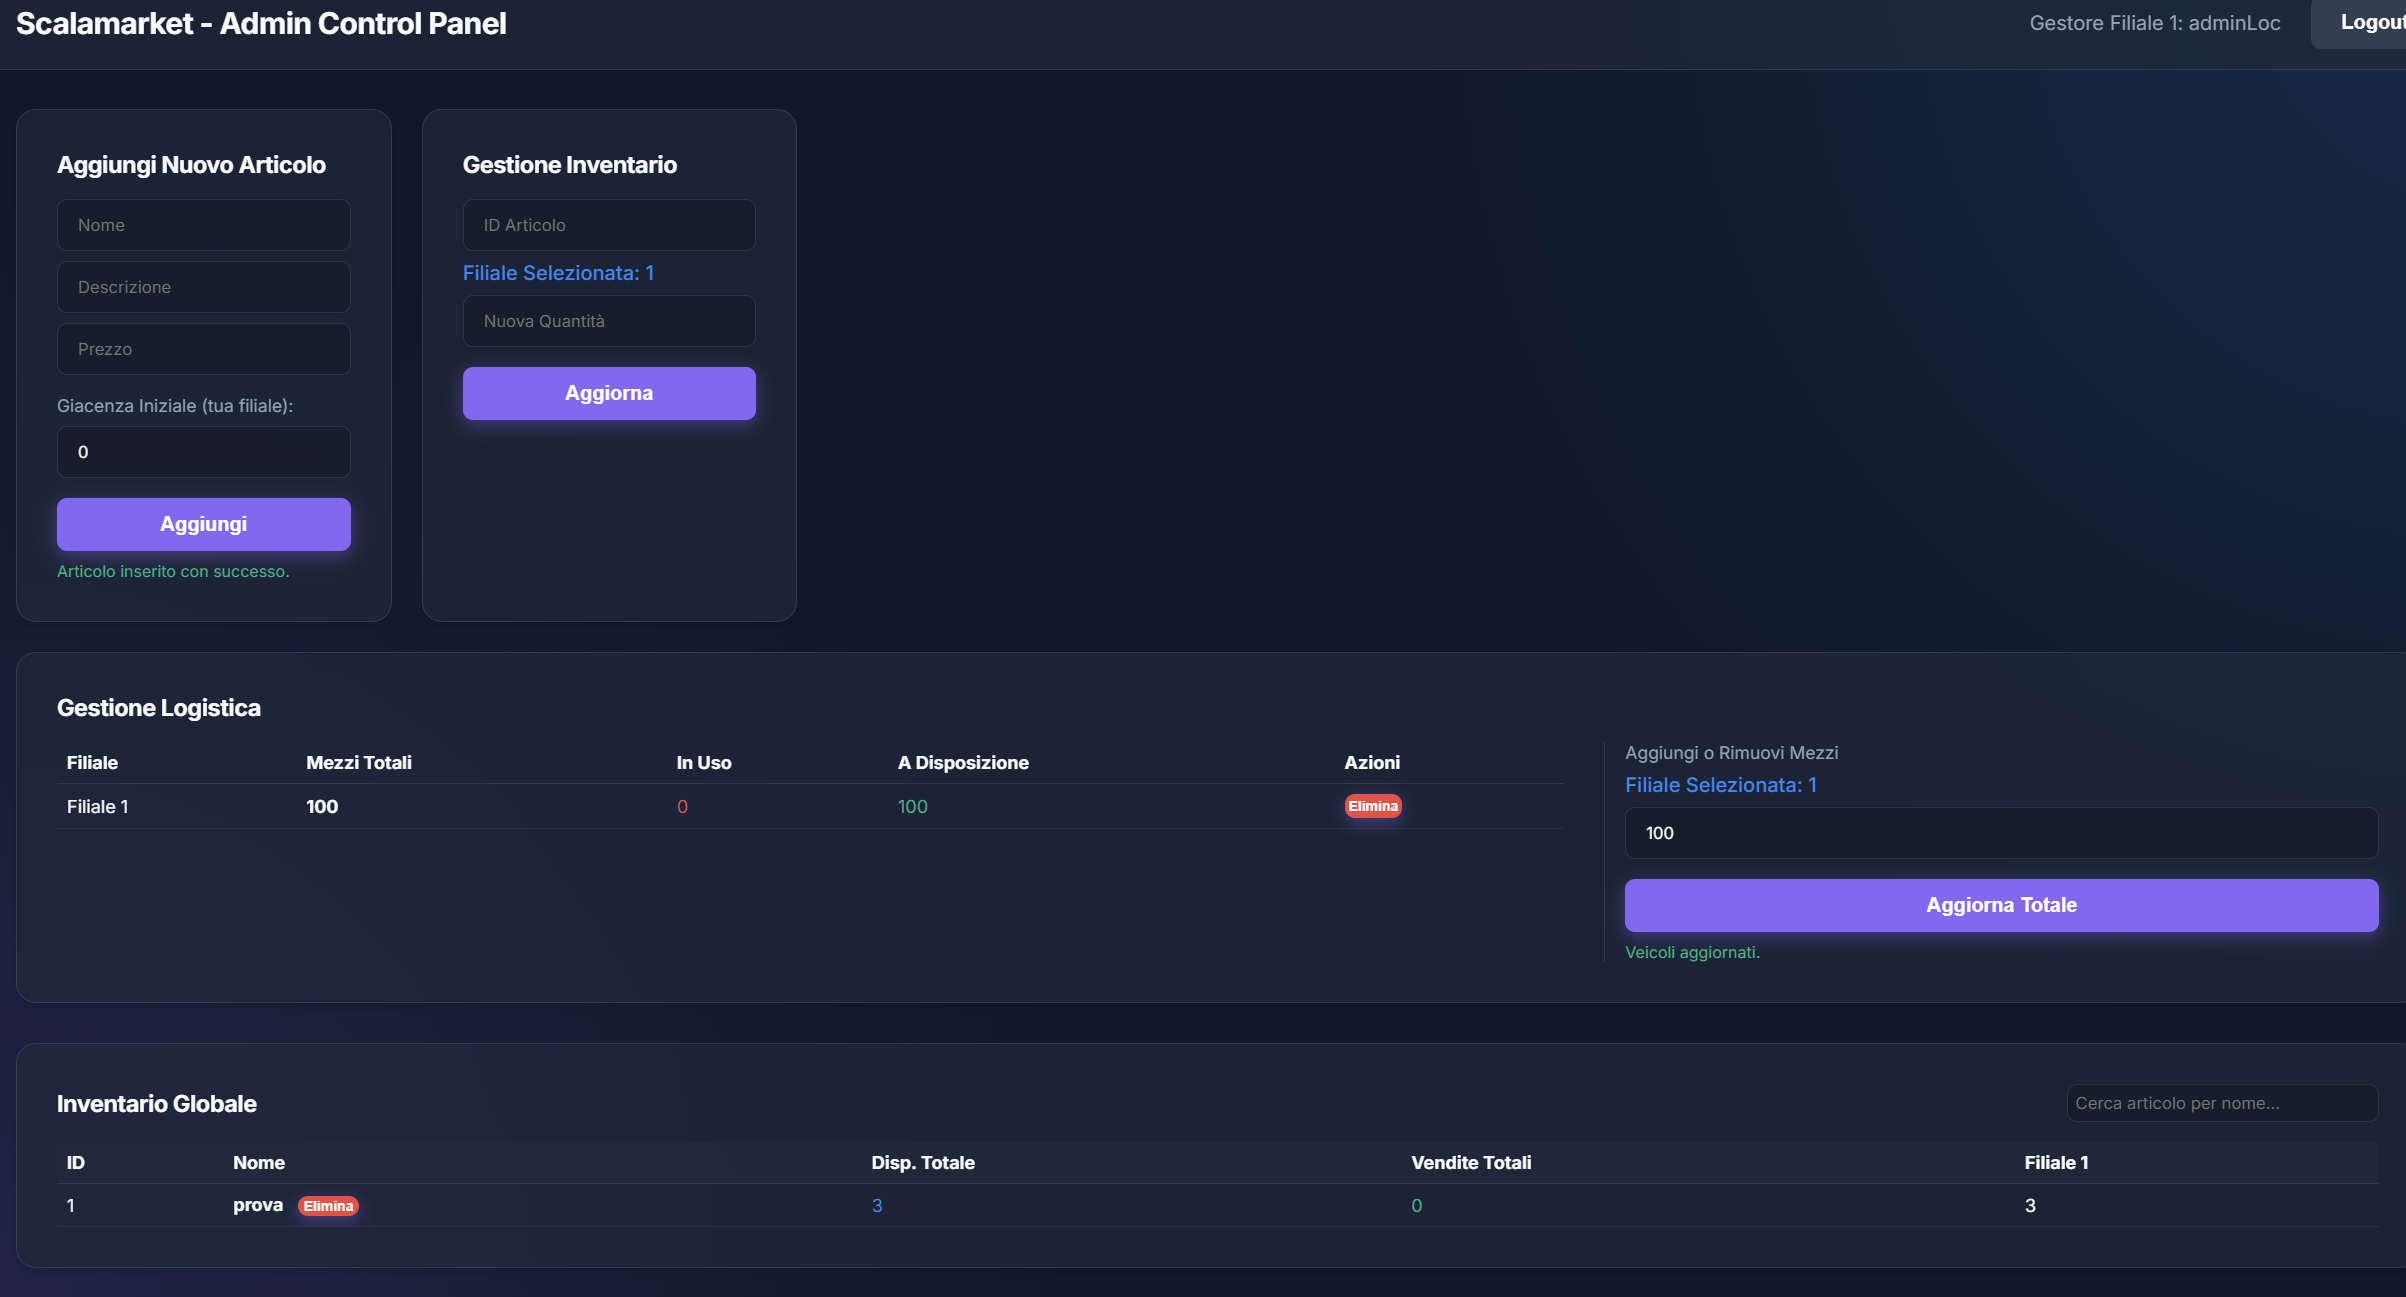
\includegraphics[width=\textwidth,height=0.45\textheight,keepaspectratio]{img/local_admin_dashboard.png}
    \caption{Dettaglio della gestione locale della singola filiale (Gestore Filiera)}
    \label{fig:local_admin_dashboard}
\end{figure}

\begin{figure}[H]
    \centering
    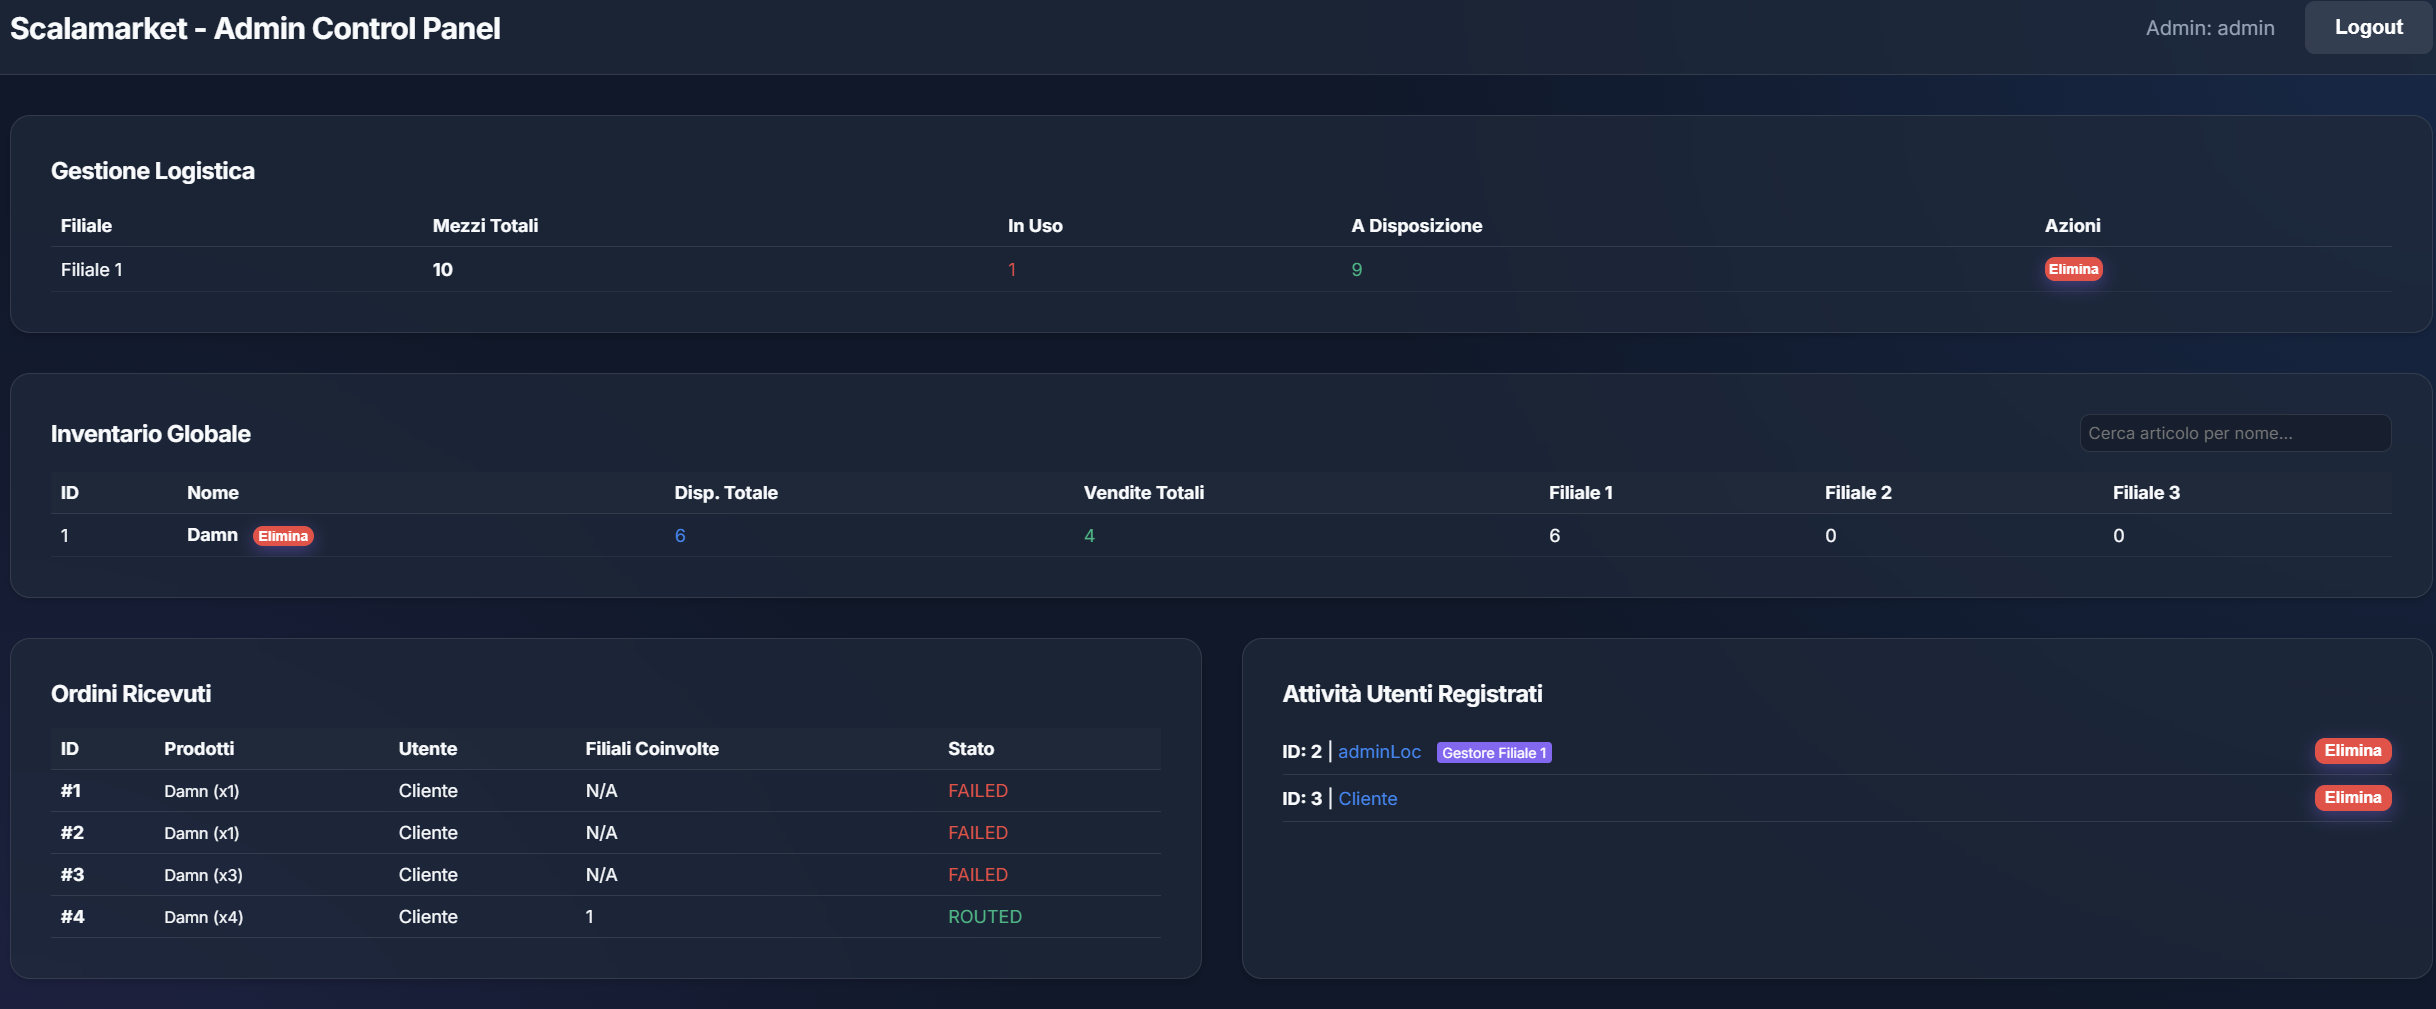
\includegraphics[width=\textwidth,height=0.45\textheight,keepaspectratio]{img/successful_order_admin.png}
    \caption{Aggiornamento in tempo reale delle risorse a seguito di un ordine}
    \label{fig:successful_order_admin}
\end{figure}

\begin{figure}[H]
    \centering
    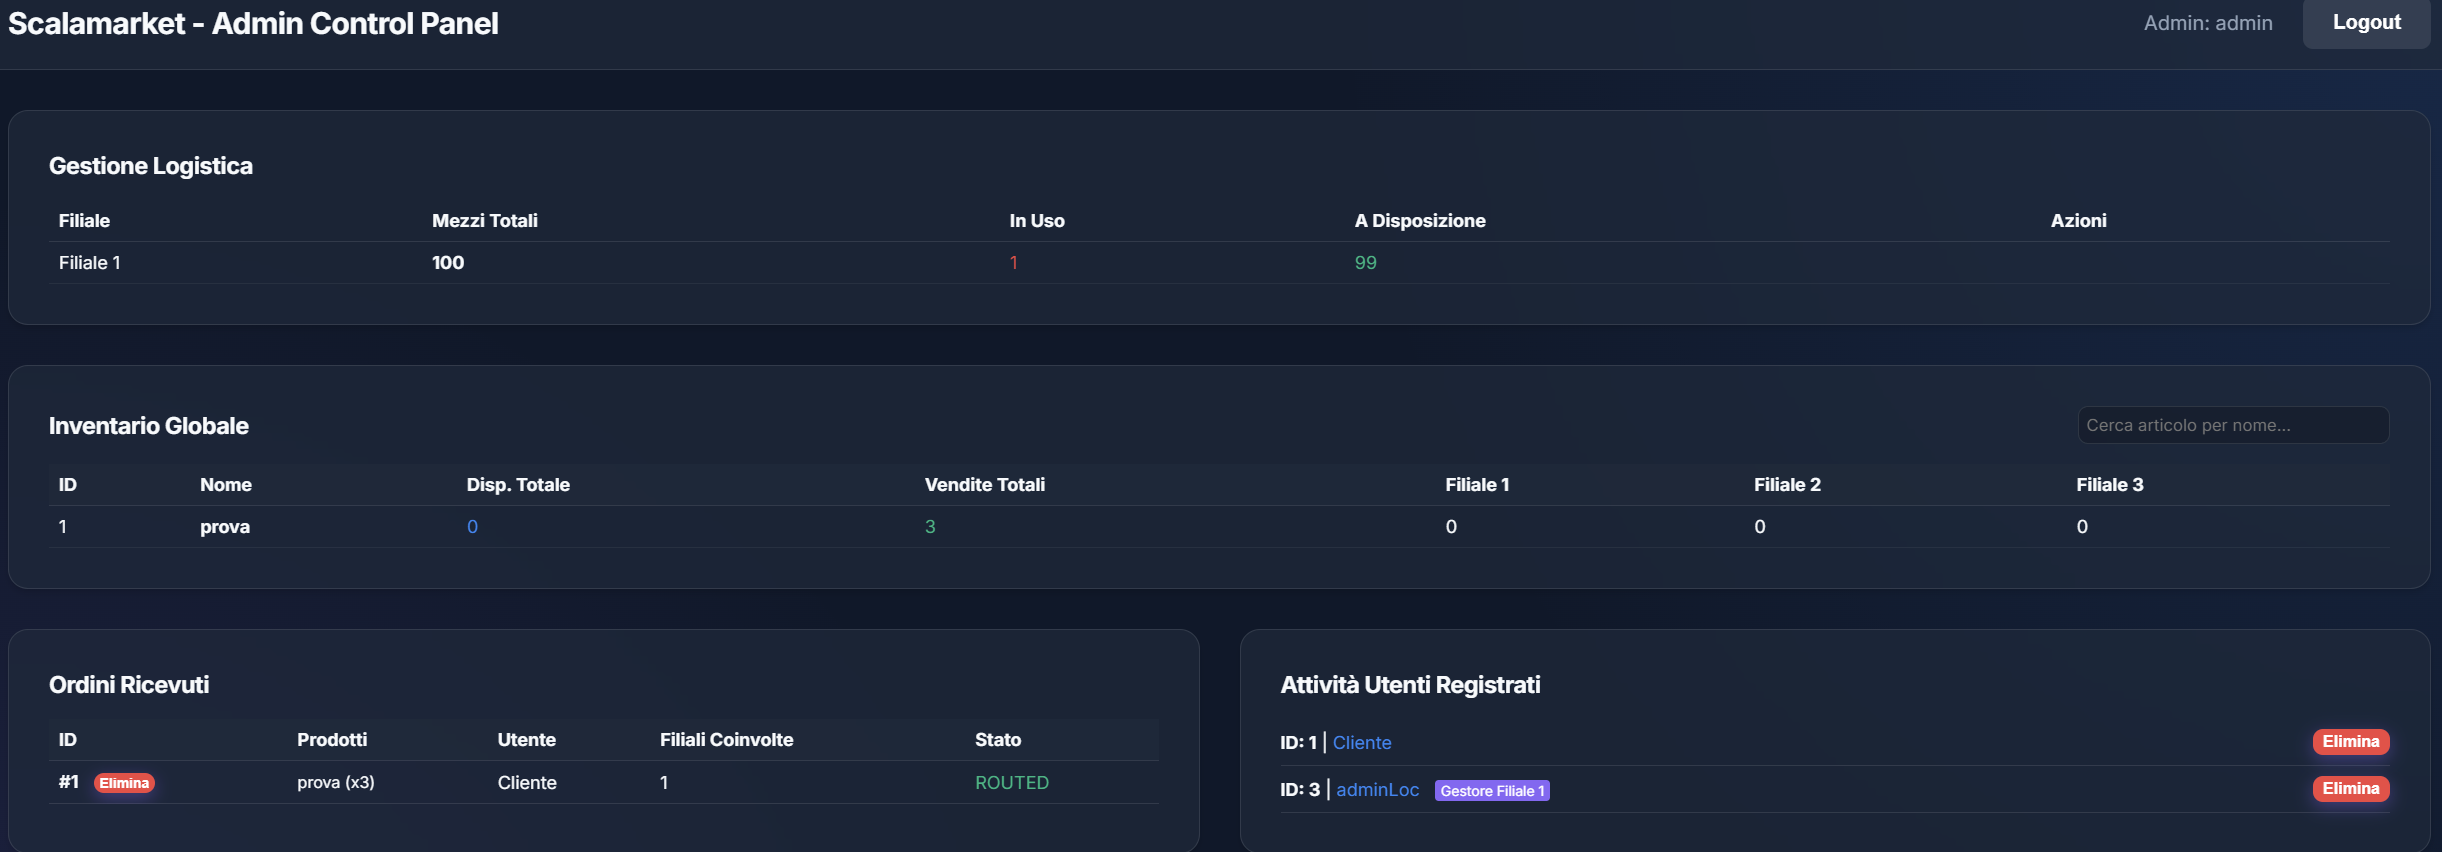
\includegraphics[width=\textwidth,height=0.45\textheight,keepaspectratio]{img/successful_order_admin_loc.png}
    \caption{Visualizzazione della ricezione dell'ordine dal pannello Gestore Filiale}
    \label{fig:successful_order_admin_loc}
\end{figure}
\end{mysection}

\end{mychapter}
